% =========================================================
% MACRO 3: DIAGRAMA DE FASES ESQUEMÁTICO (q=4)
% Uso: \qVoterPhaseDiagram{CorParamagnetica}{CorFerromagnetica}{CorDasLinhas}
% Exemplo: \qVoterPhaseDiagram{fancyBlue}{green!80!black}{red}
% =========================================================
%\newcommand{\qVoterPhaseDiagram}[5]{%
%\begin{tikzpicture}[
%    scale=\ThisScale,
%    every node/.style={font=\setBaseFont},
%    arrow/.style={-{Stealth[length={2mm*\ThisScale}, width={2mm*\ThisScale}]}, line width={1pt*\ThisScale}, black}
%]
%
%    % ==========================================
%    % 1. REGIÕES COLORIDAS (FASES)
%    % Usamos opacidade para ficar suave e não esconder os textos
%    % ==========================================
%    
%    % Região Paramagnética (Acima da curva)
%    \fill[#1, fill opacity=1] 
%        (0,6) -- (10,6) -- (10,4) parabola bend (5,2) (0,4) -- cycle;
%        
%    % Região Ferromagnética (Abaixo da curva)
%    \fill[#2, fill opacity=1] 
%        (0,0) -- (10,0) -- (10,4) parabola bend (5,2) (0,4) -- cycle;
%
%    % ==========================================
%    % 2. LINHAS DE TRANSIÇÃO
%    % ==========================================
%    
%    % Linha tracejada superior (\varepsilon = 1/4)
%    \draw[#3, dashed, line width={1.5pt*\ThisScale}] (0, 4) -- (10, 4);
%    
%    % Linha traço-ponto inferior (\varepsilon = 3/14)
%    \draw[#3, dash dot, line width={1.5pt*\ThisScale}] (0, 2) -- (10, 2);
%    
%    % Curva parabólica \bar{\varepsilon}(x)
%    \draw[#3, line width={2.5pt*\ThisScale}] (0,4) parabola bend (5,2) (10,4);
%
%    % =========================================
%    % 3. EIXOS E MARCADORES BÁSICOS
%    % ==========================================
%    
%    % Borda externa do gráfico
%    \draw[thick, line width={1pt*\ThisScale}] (0,0) rectangle (10,6);
%    
%    % Eixo X (0, 1/2, 1)
%    \foreach \x/\label in {0/-1, 5/0/2, 10/1} {
%        \draw[line width={1.5pt*\ThisScale}] (\x, 0) -- (\x, 0.2);
%        \node[below=0.5em, font=\setBaseFont\bfseries] at (\x, 0) {\label};
%    }
%    \node[below=1.8em, font=\setBaseFont\bfseries] at (5,0) {Magnetization, $\boldsymbol{\phi}$};
%    
%    % Eixo Y (Apenas indicação de \varepsilon e as frações críticas)
%    \node[right=0.1em, font=\setBaseFont\bfseries] at (0,3) {$\boldsymbol{\varepsilon}$};
%    
%    \node[right=0.2em, font=\setBaseFont\bfseries, text=#3] at (0, 4.3) {1/4};
%    \node[right=0.2em, font=\setBaseFont\bfseries, text=#3] at (0, 1.7) {3/14};
%
%    \foreach \y in {2, 4} {
%        \draw[line width={1.5pt*\ThisScale}] (0,\y) -- (0.2,\y);
%    }
%
%    % ==========================================
%    % 4. SETAS (FLUXO DA DINÂMICA)
%    % Mostram para onde o sistema vai (consenso ou desordem)
%    % ==========================================
%    
%    % Fase Paramagnética (Fluxo para o centro x=1/2)
%    \draw[arrow] (1.5, 5.0) -- (4.0, 5.0);
%    \draw[arrow] (8.5, 5.0) -- (6.0, 5.0);
%    
%    % Fase Mista (Dentro da parábola -> vai pro centro)
%    \draw[arrow] (3.0, 3.0) -- (4.5, 3.0);
%    \draw[arrow] (7.0, 3.0) -- (5.5, 3.0);
%    
%    % Fase Mista (Fora da parábola -> vai para as bordas)
%    \draw[arrow] (1.8, 2.6) -- (0.5, 2.6);
%    \draw[arrow] (8.2, 2.6) -- (9.5, 2.6);
%    
%    % Fase Ferromagnética (Fluxo para as bordas x=0 e x=1)
%    \draw[arrow] (3.5, 1.0) -- (1.0, 1.0);
%    \draw[arrow] (6.5, 1.0) -- (9.0, 1.0);
%
%    % ==========================================
%    % 5. TEXTOS DAS FASES
%    % ==========================================
%    
%    \node[font=\setBaseFont\bfseries, text=#4] at (5, 5.7) {Paramagnetic Phase};
%    \node[font=\setBaseFont\bfseries, text=#4] at (5, 5.3) {Coexistence};
%    \node[font=\setBaseFont\bfseries, text=#4] at (5, 3.6) {Mixed Phase};
%    \node[font=\setBaseFont\bfseries, text=#5] at (5, 0.9) {Consensus};
%    \node[font=\setBaseFont\bfseries, text=#5] at (5, 0.4) {Ferromagnetic Phase};
%    
%    % Rótulo da curva
%    \node[font=\setBaseFont\bfseries, text=#3] at (5, 1.6) {$\boldsymbol{\varepsilon = \bar{\varepsilon}(\phi)}$};
%
%\end{tikzpicture}%
%}

\documentclass[tikz, border=0]{standalone}
\usepackage{fontspec}
\usepackage{unicode-math}

\setmainfont{TeX Gyre Pagella}
\setmathfont{TeX Gyre Pagella Math}
\usepackage{luacode} % Pacote necessário para rodar Lua
\usetikzlibrary{calc,arrows.meta,patterns}

\definecolor{Red}{RGB}{ 159, 36, 48 }
\definecolor{Blue}{RGB}{ 103, 178, 255 }
\definecolor{LBlue}{RGB}{ 186, 220, 255 }
\definecolor{DBlue}{HTML}{132C53} 
\definecolor{gray}{HTML}{708090}
\definecolor{orange}{HTML}{ed9552}
\definecolor{orange2}{HTML}{e29d40}
\definecolor{PrintColor}{HTML}{000000}

\begin{document}


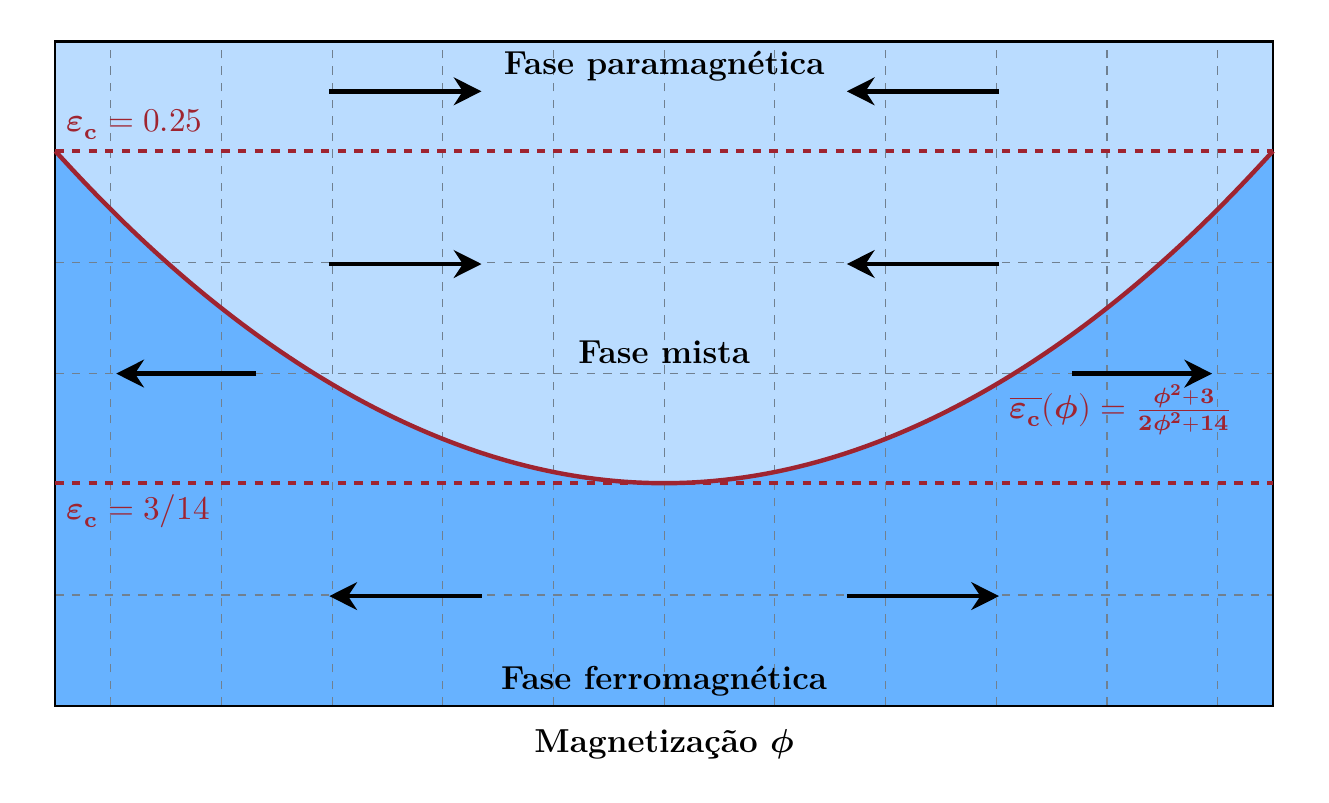
\begin{tikzpicture}[x=1em, y=1em,
        arrow/.style={-{Stealth[length=1em, width=1em]}, ultra thick, black}
]

        \def\Lx{22}
        \def\Ly{12}

        \useasboundingbox (-23,-14.5) rectangle (23,12.5);

        \coordinate (center) at (0,0);

        \coordinate (topC) at (0,\Ly);
        \coordinate (topR) at (\Lx,\Ly);
        \coordinate (topL) at (-\Lx,\Ly);
        \coordinate (topRm) at (0.5*\Lx,\Ly);
        \coordinate (topLm) at (-0.5*\Lx,\Ly);
        
        \coordinate (botC) at (0,-\Ly);
        \coordinate (botR) at (\Lx,-\Ly);
        \coordinate (botL) at (-\Lx,-\Ly);
        \coordinate (botRm) at (0.5*\Lx,-\Ly);
        \coordinate (botLm) at (-0.5*\Lx,-\Ly);

        \coordinate (leftC) at (-\Lx,0);
        \coordinate (leftTm) at (-\Lx,0.5*\Ly);
        \coordinate (leftBm) at (-\Lx,-0.5*\Ly);

        \coordinate (eps_2) at (-\Lx,0.67*\Ly);
        \coordinate (eps_1) at (-\Lx,-0.33*\Ly);
        \coordinate (eps_2R) at (\Lx,0.67*\Ly);
        \coordinate (eps_1R) at (\Lx,-0.33*\Ly);
   
        \fill[Blue] (botL) -- (botR) -- (eps_2R) parabola bend (0,-0.33*\Ly) (eps_2) -- cycle;
        \fill[LBlue] (topL) -- (eps_2) parabola bend (0,-0.33*\Ly) (eps_2R) -- (topR) -- cycle;

        % --- GRID E BORDAS ---
        \draw[step=4, dashed, gray] (botL) grid (topR);
        \draw[black, thick] (botL) rectangle (topR);

        % --- TEXTOS DAS FASES ---
        \node[font=\large\bfseries, black, anchor=north] at (topC)
            {Fase paramagnética};
        \node[font=\large\bfseries, black, anchor=south] at (center)
            {Fase mista};
        \node[font=\large\bfseries, black, anchor=south] at (botC)
            {Fase ferromagnética};
        

        % --- EIXOS ---
        \node[PrintColor, anchor=north, yshift=-0.5em, font=\large\bfseries] at (botC) {Magnetização $\symbf{\phi}$};

        \draw[arrow] (0.55*\Lx,0.85*\Ly) -- (0.3*\Lx,0.85*\Ly);
        \draw[arrow] (-0.55*\Lx,0.85*\Ly) -- (-0.3*\Lx,0.85*\Ly);

        \draw[arrow] (0.55*\Lx,0.33*\Ly) -- (0.3*\Lx,0.33*\Ly);
        \draw[arrow] (-0.55*\Lx,0.33*\Ly) -- (-0.3*\Lx,0.33*\Ly);

        \draw[arrow] (0.3*\Lx,-0.67*\Ly) -- (0.55*\Lx,-0.67*\Ly);
        \draw[arrow] (-0.3*\Lx,-0.67*\Ly) -- (-0.55*\Lx,-0.67*\Ly);

        \draw[arrow] (0.67*\Lx,0) -- (0.9*\Lx,0);
        \draw[arrow] (-0.67*\Lx,0) -- (-0.9*\Lx,0);

        \node[font=\large\bfseries, Red, anchor=south west, align=center, ultra thick]
            at (eps_2) {$\symbf{\varepsilon_c}=0.25$};
        \node[font=\large\bfseries, Red, anchor=north west, align=center, ultra thick]
            at (eps_1) {$\symbf{\varepsilon_c}=3/14$};
        
        \draw[Red, ultra thick, dashed] (eps_1) -- (eps_1R);
        \draw[Red, ultra thick, dashed] (eps_2) -- (eps_2R);

        \draw[Red, ultra thick] (eps_2) parabola bend (0,-0.33*\Ly) (eps_2R);
        
        \node[font=\large\bfseries, Red, anchor=north, align=center, ultra thick]
            at (0.75*\Lx,0) {$\symbf{\overline{\varepsilon_c}(\phi)=\frac{\phi^2+3}{2\phi^2+14}}$};

        
\end{tikzpicture}

\end{document}